\subsection{Defect Prediction}
\label{sec:defect_prediction}
%\begin{figure*}[t!]
%	\centering
%	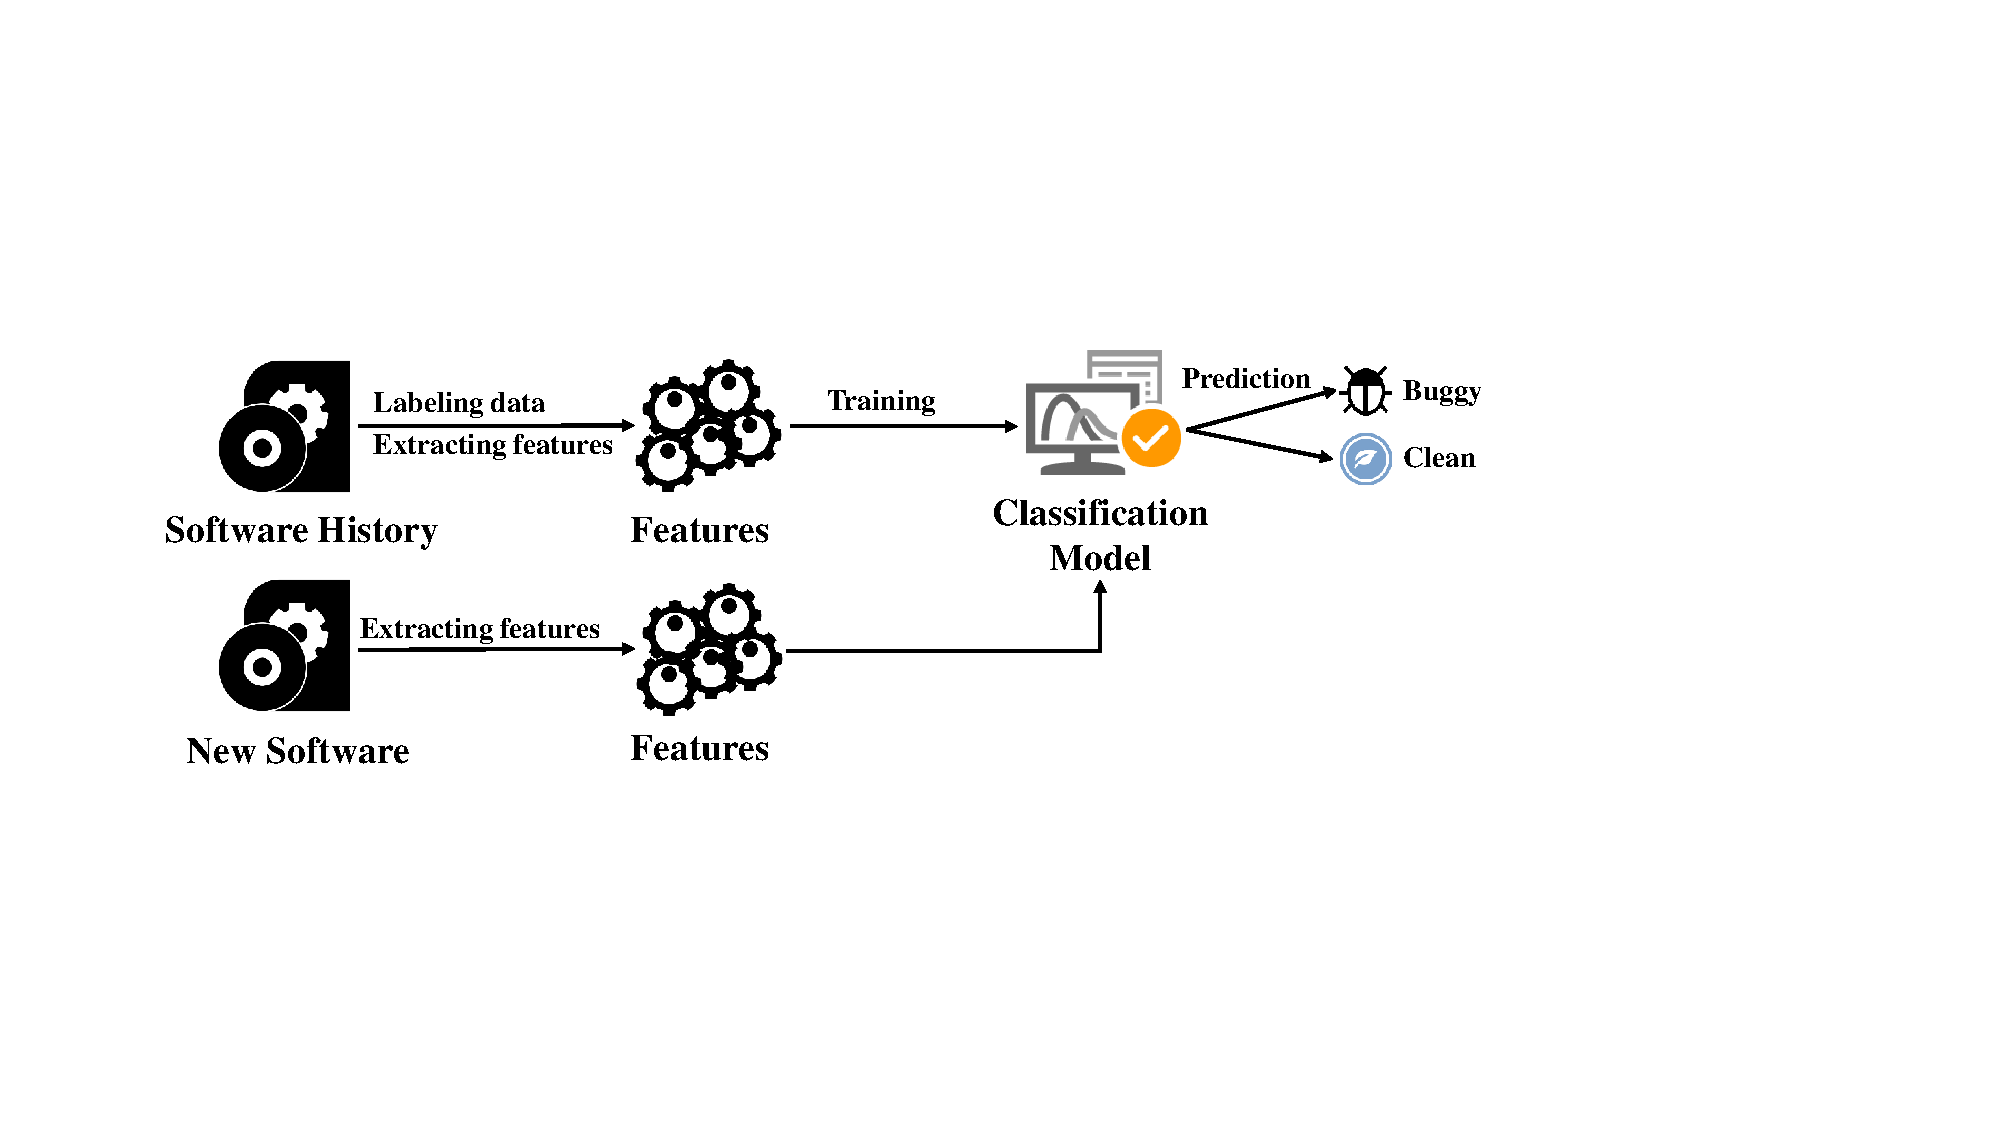
\includegraphics[width=0.85\textwidth]{defect_framework}
%	\caption{Defect Prediction Framework}
%	\label{fig:defect}
%\end{figure*}
\begin{figure}
	\centering
	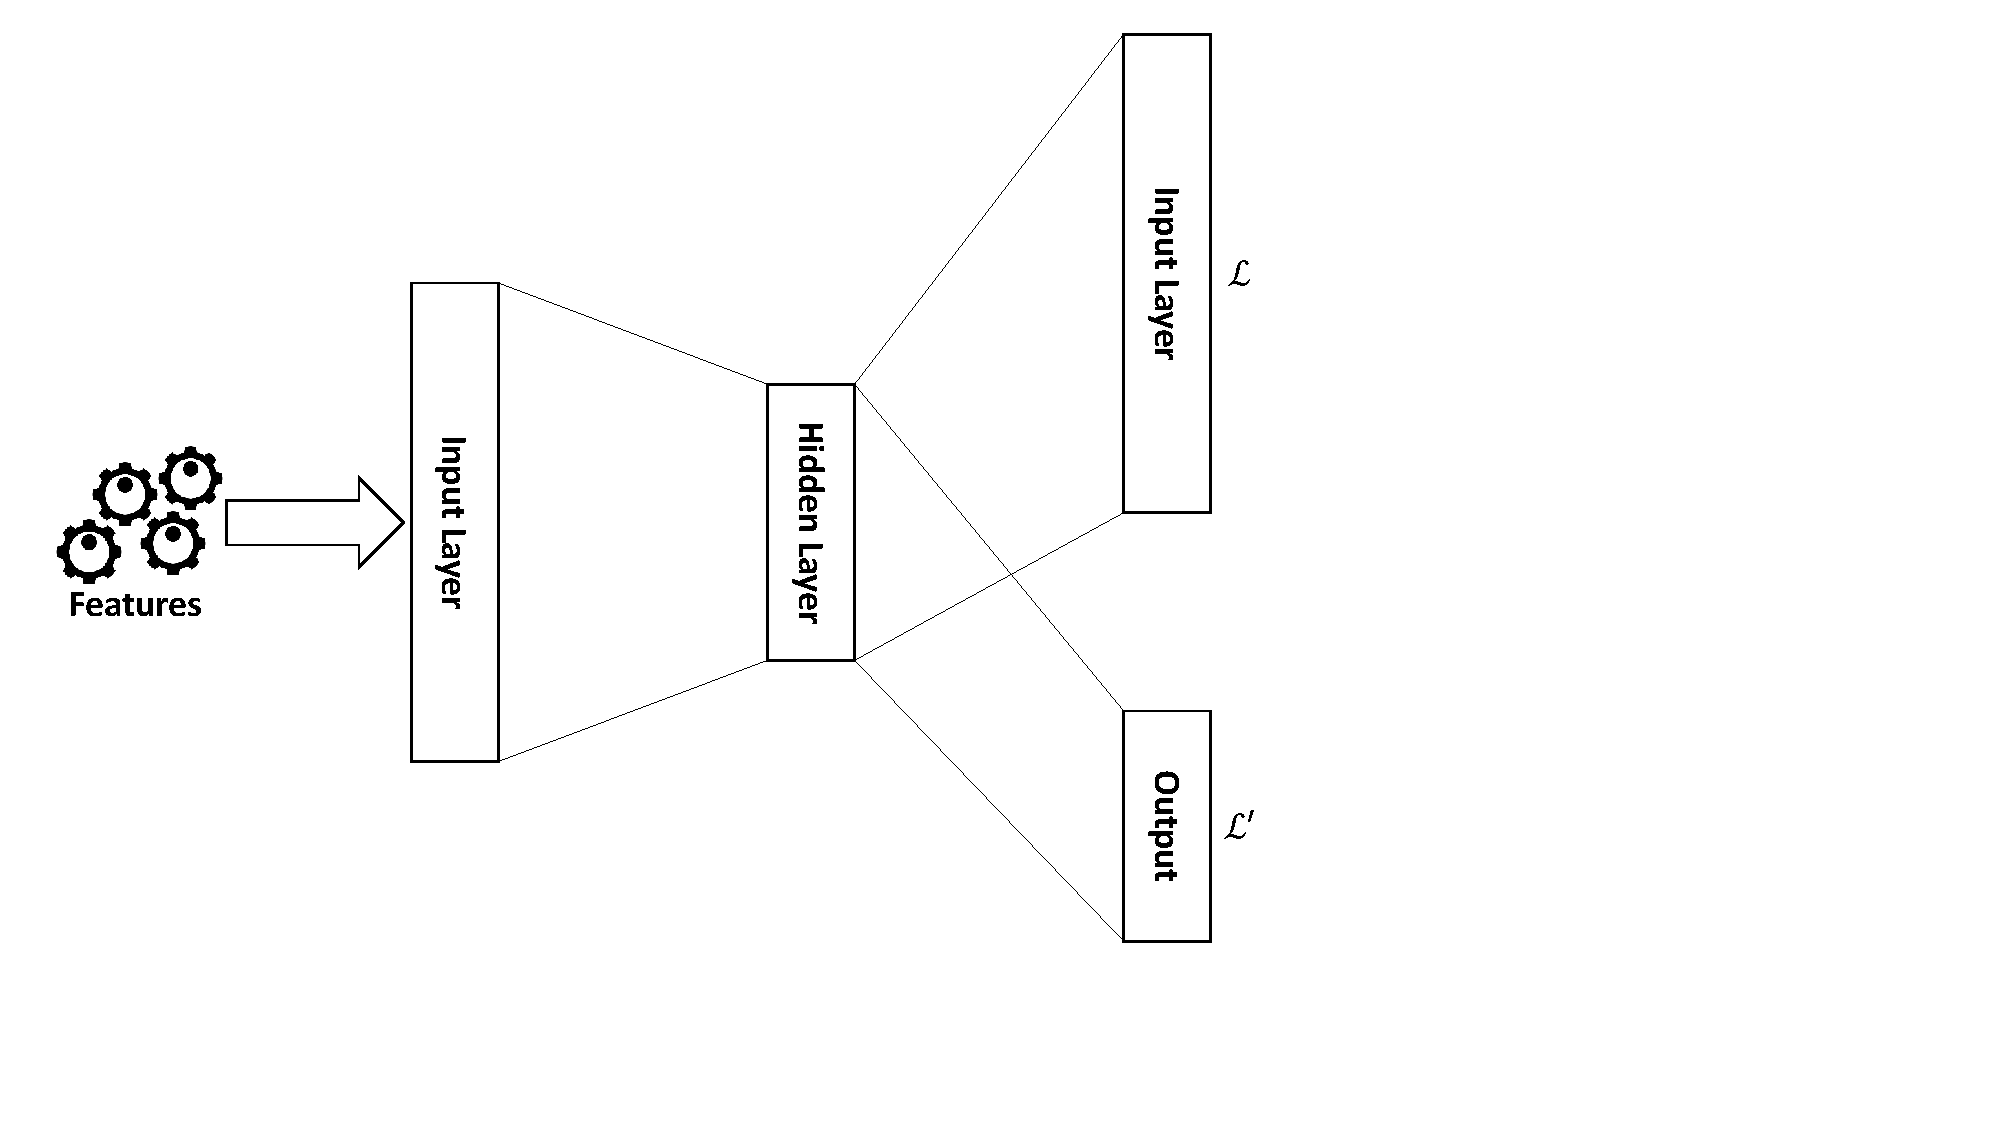
\includegraphics[width=0.45\textwidth]{dssl_framework}
	\caption{Deep Semi-supervised Learning Framework}
	\label{fig:semi_framework}
\end{figure}


%Figure~\ref{fig:defect} presents the overall framework of file-level defect prediction. Typically, the defect prediction problem is solved by following two specific steps. 
The overall process of our file-level defect prediction follows two specific steps. The first step is to label source code files as buggy or clean and then extracts traditional features of these files. These traditional features are introduced in~\cite{wang2016automatically, mccabe1976complexity, chakradeo2013mast}. The second step is to construct a defect prediction model~\cite{bishop2006pattern} to predict whether a new source code file is buggy or clean.  We refer to the software version used for building our defect prediction model as training data and the one used to evaluate the built model as testing data. 

%Figure 2 presents a typical le-level defect prediction process
%that is adopted by existing studies [20,27,34,41,42,51,
%64]. The rst step is to label data as buggy or clean based
%on post-release defects for each le. A le is buggy if the le
%contains bugs. Otherwise, the le is clean. The second step
%is to collect corresponding traditional features of these les.
%Instances with features and labels are used to train machine
%learning classiers. Finally, trained models are used to predict
%new instances as buggy or clean.
%We refer to the set of instances used for building models as
%the training set, whereas the set of instances used to evaluate
%the trained models as the test set. As shown in Figure 2,
%when performing within-project defect prediction (following
%existing work [41], we call this WPDP), the training and test
%sets are from the same project A. When performing crossproject
%defect prediction (following existing work [41] we call
%this CPDP), prediction models are trained by training set
%from a project A (source), and test set is from a dierent
%project B (target).
%In this study, we examine the performance of learned semantic
%features on both WPDP and CPDP.

\subsection{Parsing Source Code and Generating Features}
\label{sec:parsing}
%In our approach, we follow Wang et al.~\cite{wang2016automatically} to extract source code information to learn semantic features. Typically, the syntactic information from source code is collected based on Java Abstract Syntax Tree (AST)~\cite{neamtiu2005understanding}. For each program element, we extract a vector of tokens of the three types of AST nodes: 1) nodes of method invocations and class instance creations, 2) declaration nodes, i.e., method declarations, type declarations, etc. and 3) control-flow nodes such as while statements, catch clauses, if statements, for statements, etc. Note that our semi-supervised learning only takes numerical vectors as inputs, and the lengths of the input vectors are the same. Thus, we apply Wang approaches~\cite{wang2016automatically} to map between integers and tokens, and encode token vectors to integer vector. Note that our integer vectors may have different lengths, we append 0 to the integer vectors to make all the lengths consistent and equal to the length of the longest vector. We also note that adding zeros does not affect the results, since it is simply representation transformation to make the vectors acceptable by neural network~\cite{wang2016automatically}.

In our approach, we follow Wang et al.~\cite{wang2016automatically} approach to extract source code information. Typically, the syntactic information from source code is collected based on Java Abstract Syntax Tree (AST)~\cite{neamtiu2005understanding}. For each Java source code file, we extract a sequence of AST node tokens of these types: 1) nodes of method invocations and class instance creations, 2) declaration nodes, i.e., method declarations, type declarations, and enum declarations, and 3) control-flow nodes such as while statements, catch clauses, if statements, for statements, etc. Unlike Wang approach which encodes the extracted tokens as unique integers and use them as features, we encode the tokens using a term frequency - inverse document frequency (TF-IDF)~\cite{manning2008introduction} and consider them as features for our framework (i.e., deep  discriminative autoencoder). These features reflects how important a token is in its corresponding source code file.

%Note that our semi-supervised learning only takes numerical vectors as inputs, and the lengths of the input vectors are the same. Thus, we apply Wang approaches~\cite{wang2016automatically} to map between integers and tokens, and encode token vectors to integer vector. Note that our integer vectors may have different lengths, we append 0 to the integer vectors to make all the lengths consistent and equal to the length of the longest vector. We also note that adding zeros does not affect the results, since it is simply representation transformation to make the vectors acceptable by neural network~\cite{wang2016automatically}.

%DBN takes only numerical vectors as inputs, and the
%lengths of the input vectors must be the same. To use DBN
%to generate semantic features by using DBN, we rst build
%a mapping between integers and tokens, and encode token
%vectors to integer vectors. Each token has a unique integer
%identier while dierent method names and class names will
%be treated as dierent tokens. Since our integer vectors may
%have dierent lengths, we append 0 to the integer vectors
%to make all the lengths consistent and equal to the length
%of the longest vector. Adding zeros does not aect the
%results, and it is simply a representation transformation to
%make the vectors acceptable by DBN. Taking code snippets
%in Figure 3 as an example, if we consider only \File1" and
%\File2", the token vectors for \File1" and \File2" would be
%mapped to [1, 2, 3, 4] and [2, 3, 1, 4] respectively. Through
%this encoding process, method invocation information and
%inter-class information are represented as integer vectors. In
%addition, some program structure information is preserved
%since the order of tokens remains unchanged.


\subsection{Deep Semi-supervised Learning}
\label{sec:semi}
The goal of defect prediction is to detect source code files that may contain a bug in the future. 

Let $\mathcal{X}=\{x_1, x_2, \dots, x_n\}$ denotes the set of source code files in a software project and $\mathcal{Y}=\{y_1, y_2, \dots, y_n\}$ represents the set of labels for the source code files, where $n$ is the number of source code files in the project.  Note that the source code file is labeled as $1$ if it contains a bug, otherwise, it will be labeled as $0$ which means that it is clean from the bug. %The source files can be collected from github repository~\footnote{https://github.com/}
%The source files can be collected from some popular software projects (e.g, ant, camel, lucene, etc.)~\footnote{http://openscience.us/repo/defect/}. 
Unlike traditional approaches~\cite{yang2015deep, wang2016automatically} that independently learn semantic features and construct defect prediction model, our DDA approach combines the two tasks for tackling the defect prediction problem. Typically, we attempt to learn a semantic features function $f: \mathcal{X} \longmapsto \mathcal{X}$ and a defect prediction function $f': \mathcal{X} \longmapsto \mathcal{Y}$, $y_i \in \mathcal{Y}=\{0, 1\}$ indicates whether a source code file $x_i \in \mathcal{X}$ contains a bug. % which can be obtained by investigating software commit logs and bug report descriptions~\cite{fischer2003populating}.
These two functions $f$ and $f'$ can be learned by minimizing the following objective function:
%We formalize the our approaches as a joint optimization, expressed by the loss function $\mathcal{L}$, for learning semantic features and building defect prediction model as following:
\begin{equation}
\label{eq:loss}
\begin{split}
\min_{f,f'} \sum_{i}^{}\mathcal{L}(f(x_i), x_i) + \theta \mathcal{L'}(f'(x_i), y_i) \\
+ \lambda \Omega(f, f')
\end{split}
\end{equation}

where $\mathcal{L}(\cdot, \cdot)$ and $\mathcal{L}'(\cdot, \cdot)$ are the empirical loss of the semantic features and the defect prediction functions, respectively. $\theta$ is the predefined value for weighting the two loss functions. $\Omega(f, f')$ is the regularization term imposed on the two functions. The trade-off between the empirical loss and the regularization term is controlled by $\lambda$. 

The overall framework of DSSL is shown in Figure~\ref{fig:semi_framework}. The DSSL model contains three different layers: input layer, hidden layer, and output layer. Given a source code file, the features extracted in Section~\ref{sec:parsing} are fed to the input layer while the corresponding defect label is fed to the output layer. The network consisting of input layer, hidden layer, and input layer represents an encoder-decoder model. The encoder-decoder model is required to learn semantic features. Note that our encoder-decoder model are inspired by autoencoder~\cite{ng2011sparse}, which is an unsupervised learning technique. The original autoencoder only learn the function $f: \mathcal{X} \longmapsto \mathcal{X}$ so that the output values $\mathcal{\hat{X}}$ are similar to input values $\mathcal{X}$. On the other hand, DSSL attempts to learn semantic features and optimize defect prediction task, thus it takes into account two functions, i.e., $f$ and $f'$, which represents the semantic features and defect prediction function, respectively. $f'$ is learned through the connection between the hidden layer and the output layer. According to Figure~\ref{fig:semi_framework}, our model optimizes two loss functions, i.e., $\mathcal{L}$ and $\mathcal{L'}$ to construct the defect prediction model. In encoder-decoder model, we employ a fully connected neural network for learning to convert low level features from source code files to semantic features. At the same time, our network learns to determine on whether the given source code file is buggy based on the semantic features. 

%The overall framework of DSSL is shown in Figure~\ref{fig:semi_framework}. The DSSL model contains two four different parts: parsing abstract syntax tree, generating features, encoder, and decoder. The first two steps are briefly described in Section~\ref{sec:parsing} to feed source files data to our deep neural network. Encoder and decoder are required to learn semantic features as well as defect prediction model. Note that our encoder and decoder steps are inspired by autoencoder~\cite{ng2011sparse} which is an unsupervised learning technique. However the original autoencoder only tries to learn the function $f: \mathcal{X} \longmapsto \mathcal{X}$ so that the output values $\mathcal{\hat{X}}$ are similar to input values $\mathcal{X}$. However, SSA attempts to learn semantic features and optimize defect prediction model, thus it takes into account of two functions, i.e., $f$ and $f'$ represent the semantic features and defect prediction respectively. According to Figure~\ref{fig:semi_framework}, our model tries to optimize two different loss functions, i.e., $\mathcal{L}$ and $\mathcal{L'}$ to construct the defect prediction model. In encoder and decoder steps, we employ a fully connected neural network to fuse middle-level features extracted from source files to generate semantic features, where our network is learn to facilitate the determination on whether the given source code file is related to the given bug report based on the semantic features. In this paper, we employ Adam optimization~\cite{kingma2014adam}, which is popular optimization method in deep learning community, to optimize the two loss functions for constructing defect prediction model. 

%In the cross-language feature fusion layers, we employ a fully connected neural network to fuse middle-level features ex- tracted from bug reports and source files to generate a unified feature representation, where the network is learned in order to facilitate the determination on whether the given source code file is related to the given bug report based on the uni- fied feature.


%To learn semantic features from program elements, we employ autoencdoer

%Ω(f) is a regulariza- tion term imposing on the prediction function. The trade-off between L(·, ·) and Ω(f ) is balanced by λ.

%Let C = fc1; c2;    ; cN1g denotes the set of source code
%files of a software project andR = fr1; r2;    ; rN2g denotes
%the collection of bug reports received by the software maintenance
%team, where N1;N2 are the number of source files and
%bug reports, respectively. The bug reports and source files can
%be collected from bug tracking systems (e.g., Bugzilla, Jira,
%etc.) and history control systems (e.g., CVS, Git, etc.).

\subsection{Imbalanced Problem in Defect Prediction}
\label{sec:imbalanced}
In defect prediction tasks, often times there are only a few source code files that contain bugs while the other source code files are \textit{clean}~\cite{khoshgoftaar2010attribute}. This consequently makes the labeled data to be imbalanced. This imbalanced nature increases the learning difficulty. For this reason, imbalanced class learning, which specializes in tackling classification problems involving imbalanced data, is helpful for defect prediction problem~\cite{wang2013using}. To address this imbalanced data issue, we propose a balanced random sampling procedure when picking a data instance to update our DSSL network weights. In particular, we select a random instance from each the positive and negative instance pools to mitigate the issue of skewed distribution. This mitigates the issue of imbalanced data in defect prediction. 


%To address this problem, we propose to learn the semantic features that may counteract the negative influence of the imbalanced data in the subsequent learning of defect prediction function. Inspired by~\cite{zhou2006training}, we introduce an unequal misclassification cost according to the imbalance ratio and train the fully connected network in a cost-sensitive manner. 
%
%Let $r_n$ denote the ratio cost of incorrectly associating an \textit{clean} source code file to a bug program element and $r_p$ denote the cost of missing a buggy source code file in the training data. The weight of the semi-supervised autoencoder (SSA) networks $\mathcal{W}$  can be learned by minimizing the following objective function following Adam optimization~\cite{kingma2014adam}. 
%\begin{equation}
%\label{eq:imbalanced}
%\begin{split}
%\min_{\mathcal{W}} \sum_{i}^{}\mathcal{L}(f(x_i), x_i) 
%+ r_n \mathcal{L}'(x_i, y_i;\mathcal{W}) y_i \\ + r_p \mathcal{L}'(x_i, y_i;\mathcal{W}) (1 - y_i) + \lambda \rVert \mathcal{W} \rVert^2
%\end{split}
%\end{equation}
%where $\mathcal{L}$ and $\mathcal{L}'$ are the loss function for semantic features and defect prediction model, respectively. $\lambda$ is the trade-off parameter.  
%To address this, we devise a balanced random
%sampling procedure when picking a data instance for gradient
%descent update. In particular, for every update step, we
%alternatingly select a random instance from the positive and
%negative instance pools, as per lines 4-8 of Algorithm 1.
%Using this simple method, we can balance the training
%from positive and negative instances, thus effectively mitigating
%the issue of skewed distribution in the localization
%task. It is also worth noting that our iterative tuning procedure
%is efficient. That is, its time complexity is linear with
%respect to the number of instances N and maximum iterations
%Tmax.


%Let costn denote the cost of incorrectly associating an ir- relevant source code file to a bug report and costp denote the cost of missing a buggy source code file that is responsible for the reported bugs. The weight of the fully connected net- works w can be learned by minimizing the following objec- tive function based on SGD (stochastic gradient descent).

%the imbalanced nature of this type of data increases the learning difficulty of such a task. Class imbalance learning specializes in tackling classification problems with imbalanced distributions, which could be helpful for defect prediction, but has not been investigated in depth so far. In this paper, we study the issue of if and how class imbalance learning methods can benefit software defect prediction with the aim of finding better solutions.    



%In the cross-language feature fusion layers, we employ a fully connected neural network to fuse middle-level features ex- tracted from bug reports and source files to generate a unified feature representation, where the network is learned in order to facilitate the determination on whether the given source code file is related to the given bug report based on the uni- fied feature.
%In most cases of bug localization, a reported bug may be only related to one or only a few source code files, while a large number of source code files are irrelevant to the given bug report. Such an imbalance nature increases the difficulty in learning a well-performing prediction function based on the unified feature.
%To address this problem, we propose to learn the unified feature that may counteract the negative influence of the im- balanced data in the subsequent learning of prediction func- tion. Inspired by [Zhou and Liu, 2006], we introduce an un- equal misclassification cost according to the imbalance ratio and train the fully connected network in a cost-sensitive man- ner.
%Let costn denote the cost of incorrectly associating an ir- relevant source code file to a bug report and costp denote the cost of missing a buggy source code file that is responsible for the reported bugs. The weight of the fully connected net- works w can be learned by minimizing the following objec- tive function based on SGD (stochastic gradient descent).

\subsection{Setting for Training Deep Semi-supervised Learning}
\label{sec:setting}
In our setting, the number of hidden layers, the number of nodes in each hidden layer, the number of iterations, and $\theta$ are chosen by performing cross validation on training data. By default, the number of hidden layers, the number of nodes in each hidden layer, and number of iteration are selected as 2, 1000-100, and 75, respectively. We employ Adam optimization~\cite{kingma2014adam}, which is popular optimization method in deep learning community, to optimize the two loss functions for constructing DSSL. %Note that $\theta$ in Equation~\ref{eq:loss} is also well-chosen based on training data to solving imbalanced between two loss functions. 


%Some deep learning application~\cite{hinton2009deep, ng2011sparse} reports an effective of deep learning models need well-tuned parameters, i.e., 1) the number of hidden layers, 2) the number of nodes in each hidden layer, and 3) the number of iterations.
%In our deep  discriminative autoencoder, we choose two hidden layers and  these parameters are chosen by learning from training data 
%
% In~\cite{wang2016automatically}, the authors pointed out that the deep learning model was optimized when they chose 10, 100, 200 as the number of hidden layers, number of nodes in each hidden layer, and number of iterations respectively. For the fair comparison with~\cite{wang2016automatically}, we use these parameters to train our DDA model. 

%Many DBN applications [6,25,37] report that an eective
%DBN needs well-tuned parameters, i.e., 1) the number of hid-
%den layers, 2) the number of nodes in each hidden layer, and
%3) the number of iterations. In this study, since we leverage
%DBN to generate semantic features, we need to consider the
%impact of the three parameters. We tune the three parameters
%by conducting experiments with dierent values of the
%parameters on ant (1.5, 1.6), camel (1.2, 1.4), jEdit (4.0,
%4.1), lucene (2.0, 2.2), and poi (1.5, 2.5) respectively. Each
%experiment has specic values of the three parameters and
%runs on the ve projects individually. Given an experiment,
%for each project, we use the older version of this project to
%train a DBN with respect to the specic values of the three
%parameters. Then, we use the trained DBN to generate semantic
%features for both the older and newer versions. After
%that, we use the older version to build a defect prediction
%model and apply it to the newer version. Lastly, we evaluate
%the specic values of the parameters by the average F1 score
%of the ve projects in defect prediction.



